\normalfalse \difficilefalse \tdifficiletrue
\correctionfalse

%\UPSTIidClasse{11} % 11 sup, 12 spé
%\newcommand{\UPSTIidClasse}{12}

\exer{Variateur de Graham\ifprof\else\footnote{Les éventuelles erreur de texte font partie intégrante de la difficulté :).}\fi $\star\star\star$ \label{C2:09:19}}
\begin{flushright}
\textit{D'après ressources de Michel Huguet.}
\end{flushright}
\setcounter{question}{0}\UPSTIcompetence[2]{C2-09}
\index{Compétence C2-09}
\index{TEC}
\index{Théorème de l'énergie cinétique}
\index{Variateur de Graham}
\ifcorrection
\else
\textbf{Pas de corrigé pour cet exercice.}
\fi

\ifprof
\else

Soit le schéma suivant. 
\begin{center}
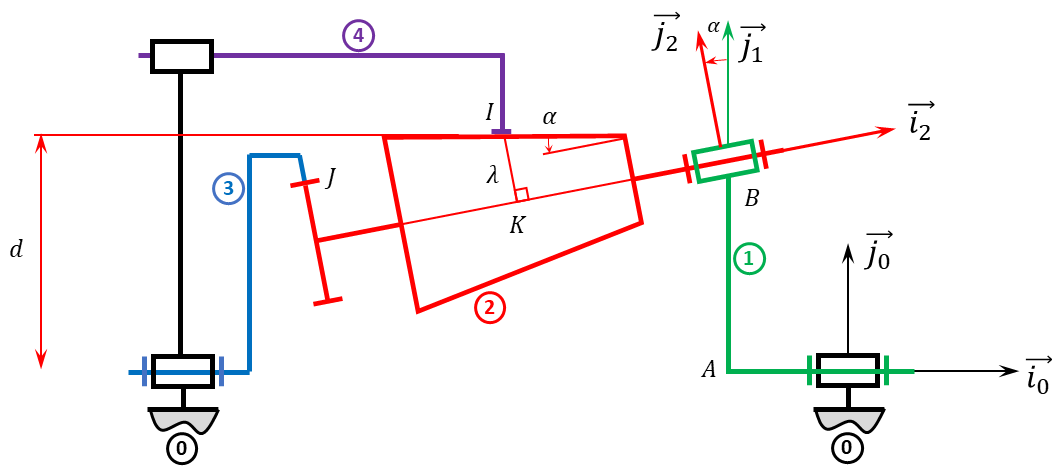
\includegraphics[width=\linewidth]{19_01}

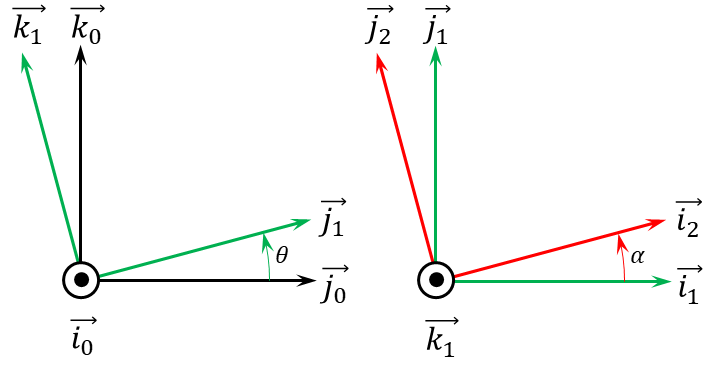
\includegraphics[width=\linewidth]{19_02}
\end{center}

On note
$\vect{AJ}=-L \vect{i_0}+\dfrac{d_3}{2}\vect{j_2}$
et 
$\vect{KJ}=-\ell \vect{i_2}+\dfrac{d_2}{2}\vect{j_2}$.

Soit $\rep{}=\repere{A}{i_0}{j_0}{k_0}$ un repère lié au bâti \textbf{0} du variateur. L’arbre moteur \textbf{1} et l’arbre récepteur
\textbf{3} ont une liaison pivot d’axe $\axe{A}{i_0}$ avec le bâti \textbf{0}. On pose $\vecto{1}{0}=\omega_1\vect{i_0}$ et $\vecto{3}{0}=\omega_3\vect{i_0}$. 

Soit $\rep{1}=\repere{A}{i_0}{j_1}{k_1}$  et $\rep{2}=\repere{B}{i_2}{j_2}{k_1}$ deux repères liés respectivement à \textbf{1} et \textbf{2} tels que $\vect{AB}$ ait même direction que  $\vect{j_1}$. On pose $\alpha =  \angl{i_1}{i_2}$ constant. 

Le satellite \textbf{2} a une liaison pivot d’axe $\angl{B}{i_2}$ avec \textbf{1}. \textbf{2} est un tronc de cône de
révolution d’axe $\angl{B}{i_2}$ de demi angle au sommet $\alpha$. On pose $\vecto{S_2}{S_1}=\omega\vect{i_2}$.

La génératrice de \textbf{2} du plan $\left(O,\vect{i_0},\vect{j_1} \right)$  la plus éloignée de l’axe $\axe{O}{i_0}$
 est parallèle à $\vect{i_0}$. Notons $d$ sa distance à l’axe $\axe{O}{i_0}$

\textbf{2} roule sans glisser au point $I$, sur une couronne \textbf{4}, immobile par rapport à \textbf{0} pendant le
fonctionnement. Le réglage du rapport de variation s’obtient en déplaçant \textbf{4} suivant l’axe
$\axe{O}{i_0}$.

Soit $K$ le centre de la section droite du tronc de cône passant par $I$. On pose $\vect{BI}=\lambda{j_2}$.
À l’extrémité de \textbf{2} est fixée une roue dentée de $n$ dents, d’axe $\axe{B}{i_2}$, qui engrène avec une
couronne dentée intérieure d’axe $\axe{A}{i_0}$, de $n_2$ dents, liée à \textbf{3}.
\fi


\question{Tracer le graphe des liaisons.}
\ifprof
\else
\fi

\question{En exprimant que \textbf{2} roule sans glisser sur \textbf{4} au point $I$, déterminer $\omega$ en fonction de $\omega_1$,
d et $\lambda$.}
\ifprof
\else
\fi

\question{Quelle relation obtient-on entre $\omega_1$, $\omega_3$ et $\omega$ en exprimant l’engrènement des deux roues
dentées ? (c’est à dire que \textbf{2} et \textbf{3} roulent sans glisser l’un sur l’autre en $J$).}
\ifprof
\else
\fi

\question{En déduire le rapport de variation $\dfrac{\omega_3}{\omega_1}$ du mécanisme en fonction de $\lambda$, $d_2$, $d_3$ et $d$.}
\ifprof
\else
\fi

\question{Tracer la courbe représentative du rapport de variation $\dfrac{\omega_3}{\omega_1}$ du mécanisme en fonction de $\lambda$, sachant que $\dfrac{n}{n_3}=\dfrac{d_1}{d_3}$, $d=\SI{55}{mm}$ et que $\lambda$ varie entre 
$\lambda_{\text{mini}}=\SI{12}{mm}$ et la valeur
$\lambda_{\text{maxi}}=\SI{23}{mm}$.}
\ifprof
\else
\fi


\ifprof
\else
\begin{flushright}
\footnotesize{Corrigé  voir \ref{C2:09:19}.}
\end{flushright}%
\fi